\newpage\null\thispagestyle{empty}\newpage
\chapter{Metodologia}
\label{chap:metod}

Neste capítulo serão apresentadas as adaptações das metodologias e técnicas
definidas para o desenvolvimento deste trabalho. As seções estão dispostas
em:

\begin{enumerate}
  \item \textbf{Levantamento Bibliográfico}: define os métodos utilizados nas
    pesquisas e levantamento bibliográfico;
  \item \textbf{Escolha de Tecnologias}: mostra as tecnologias e
    ferramentas de suporte e dependentes ao desenvolvimento do trabalho;
  \item \textbf{Análise do Ambiente}: mostra o modo de definição das camadas e os critérios para
    a seleção da mesma;
  \item \textbf{Definição dos Recursos Chef}: mostram o modo de escolha dos recurso do Chef a serem utilizados;
  \item \textbf{Metodologia de Desenvolvimento} que mostra o métodos e práticas da engenharia de software
    definidos para serem utilizados no desenvolvimento do trabalho;
  \item \textbf{Coleta e Análise de Resultados} que mostra como será feito a validação da proposta.
\end{enumerate}

\section{Levantamento Bibliográfico}

Para o referenciamento desse trabalho, foram levantados estudos a cerca de
\mbox{DevOps}, Chef, Infraestrutura como Código e outros assuntos relevantes com
auxílio do Periódico Capes, Google Acadêmico dentre outras fontes.
Apesar de serem assuntos recentes, existe muita discussão e pesquisa a
respeito deles. Há muitas aplicações desses conceitos, principalmente
em empresas de software de renome como Google, Facebook, Apple, em
empresas recentes e em \textit{start-ups}. Dessa forma, existem muitas publicações e %TODO: (Dessa forma...)sem uma referencia isso não deveria ser dito
palestras nos canais usados por essas empresas e grupos, para divulgar
experiências e conhecimentos a respeito desses assuntos e essas fontes
também foram utilizadas para referenciar esse trabalho.

%TODO: colocar o método de levantamento e o tipo de pesquisa



\section{Escolha de Tecnologias}
\label{sec:tec}

%TODO: a seção explica o motívo e critérios utilizados para escolher as tecnologias.

Já que a aplicação proposta por este trabalho (Cupper) tem a intenção de entrar
na família de ferramentas relacionadas ao Chef, é interessante que ela seja uma
Gem, ou seja, que seja desenvolvida na linguagem Ruby e seja disponibilizada pelo %TODO: frase estranha
gerenciador de pacotes RubyGems, estando no padrão das outras ferramentas da
família Chef.

A decisão pelo próprio Chef vem da experiência que o grupo tem com essa ferramenta.
Por já estarem familiarizados com a estrutura, sintaxe e formas de execução do Chef,
a escolha do Chef para a ferramenta de gerência e configuração de ambientes foi a
mais natural. %TODO: essa afirmação é válida?

Por mais que o Chef esteja relacionado ao desenvolvimento do Cupper, ele não é uma
dependência para a execução do mesmo, e sim uma ferramenta que usa a saída do Cupper
para outro fim, como será explicado no capítulo \ref{chap:desenv}, de Desenvolvimento.
Uma dependência que foi levantada para o desenvolvimento do Cupper é o Ohai,
outra ferramenta da família Chef, que será necessária para fazer o perfil e diagnóstico
inicial do sistema. %TODO: melhorar

\section{Ferramentas e Serviços de Suporte ao Desenvolvimento}

Para o desenvolvimento do trabalho, foram escolhidas as ferramentas e serviços de suporte que serão
utilizadas para gerência e controle das atividades do projeto e automação e coleta de dados e teste
de desenvolvimento do Cupper. A escolha foi feita considerando a experiência do
grupo em relação a utilização da ferramenta no decorrer do curso e a identificação dos
padrões utilizados pelas ferramentas providas pelo Chef.

\subsection{Git}

Git é uma ferramenta de controle de versão gratuita e de código aberto criada
em 2005 por Linus Torvalds~\cite{chacon:2014}. O Git foi utilizado para o controle das versões
dos códigos para a produção deste documento e para a produção da ferramenta proposta Cupper.

\subsection{Github}

O Github é um serviço que provê a utilização dos comando Git em um \textit{browser}, além de
disponibilizar um repositório remoto para colaboração de projetos e registro e rastreamento de
\textit{issues}~\cite{github:2016}.  O Github foi utilizado para armazenamento remoto do repositório
deste documento e da ferramenta proposta Cupper, e para o registro e controle de \textit{issues} que são
considerados os itens do \textit{Backlog}, como descrito na seção~\ref{sec:praticas_tecnicas}.

\subsection{Travis}

O Travis é um serviço de integração contínua integrada com o serviço Github que automatiza
a \textit{build} do código e verifica os testes~\cite{travis:2016}. O Travis será utilizado para
realizar a \textit{build} automatica da ferramenta Cupper, determinando se a funcionalidade ou \textit{bugfix}
será integrada ao código.

\subsection{RubyGems}

O RubyGems é um \textit{framework} de empacotamento e instalação de bibliotecas e aplicações
construidas com Ruby. As vantagens de se utilizar RubyGem~\cite{thomas:2001}:

\begin{itemize}
 \item Padronizar formatos de pacotes;
 \item Centralizar o repositório para distribuição dos pacotes Gem;
 \item Facilitar a instalação, gerenciamento e manipulação dos pacotes Gem.
\end{itemize}

A ferramenta Cupper, por ser construída em Ruby, seguirá os padrões adotados
pelo RubyGems.

\subsection{RSpec}

O RSpec é um \textit{framework} de \textit{Behaviour-Driven Development} (BDD)
criado por Steven Baker em 2005~\cite{chelimsky:2010}. Com o RSpec
são criados testes que descrevem um comportamento esperado do sistema
em contexto controlados. O RSpec facilita a escrita de testes simplificando
a sintaxe para descrever os cenários e comportamentos.

\section{Ferramentas Dependentes}

Foram identificadas as ferramentas dependentes para a construção do Cupper.
São ferramentas que estão dentro da família de ferramentas do Chef e são
de código aberto disponíveis no repositório oficial do Chef.

\subsection{Ohai}

O Ohai é uma ferramenta para detecção de atributos de um \textit{node}. Os atributos são
informações que podem ser: detalhe de plataforma, dados de CPU, dados de redes, etc.
O Ohai é uma dependência do \textit{chef-client} e é extensível através de \textit{plugins}
para incluir mais tipos de dados a serem coletados~\cite{ohaidoc:2016}.

Para o desenvolvimento do Cupper, a ferramenta Ohai será utilizada para realizar a
interface de coleta de dados. Como será apresentado na seção~\ref{sec:cam-amb}, o
Ohai, sem extensões, pode coletar uma certa quantidade de atributos do ambiente, sendo
necessário a criação de \textit{plugins} de acordo com a necessidade de implementação do Cupper.


\section{Análise do Ambiente}

Neste trabalho, é considerado como ambiente uma máquina composta
de hardware e sistema operacional. São consideradas máquinas físicas
e virtuais. Essa seção irá descrever como será a análise e extração
de informações do ambiente.

\subsection{Definição de Camadas}

Para decidir até que ponto a aplicação irá analisar as configurações
do ambiente é preciso definir os tipos de configuração, as características para
cada, e separar esses tipos em camadas onde a aplicação pode atuar.
Com essas camadas definidas, identifica-se quais camadas são relevantes e viáveis
para o escopo do trabalho.

%TODO: adicionar como foi feita a definição das camadas

\subsection{Definição de Critérios para a Seleção}
\label{sec:defcritcamada}
Após levantar as camadas de configuração do ambiente, é necessário definir em
quais camadas e em quais dos seus atributos o Cupper realmente vai atuar. 
Os critérios vão estar relacionados a dois aspectos importantes: a \textbf{relevância} 
para o projeto e a quantidade de \textbf{esforço} e \textbf{tempo} para a implementação durante
o Trabalho de Conclusão de Curso.

Para classificar um atributo como relevante para análise, ele deve seguir os
seguintes critérios:

\begin{enumerate}
\item Um atributo é relevante quando ele é necessário para a geração de uma
receita Chef que atenda aos nossos requisitos. 

Na seção~\ref{sec:lev-rec} e~\ref{sec:escopo} definimos os recursos Chef
que iremos utilizar nas criações de \textit{cookbooks} e até que ponto 
avançaremos nas funcionalidades do Cupper, e dessa forma, os atributos
são relevantes se eles se enquadram nesse patamar, para alcançar esses objetivos.

Um exemplo básico disso é a arquitetura da CPU, que pode alterar a instalação
e qual a versão de pacotes a serem instalados.

\item Um atributo também é relevante se é necessário para criação de \textit{logs} 
e \textit{debugs}, tanto para uso da ferramenta durante o processo de gerar 
\textit{cookbooks} quanto para algum retorno para o usuário, para ajudar 
a entender possíveis erros ao executar
o Cupper.
\end{enumerate}

Com relação à dificuldade de implementação e de integração ao Cupper o
atributo deve seguir os seguinte critérios em ordem de prioridade:

\begin{enumerate}
\item O atributo tem maior prioridade de ser selecionado se é um dos dados 
que o Ohai lança por padrão e sem extensões.
\item O atributo tem média prioridade se, não é um dos dados que o Ohai
lança por padrão e sem extensões, mas existe um comando do sistema que facilita 
sua extração, e dessa forma facilitando a criação de \textit{plugins} pro 
Ohai.
\item O atributo tem menor prioridade se não é lançado pelo Ohai e nem tem 
comandos do sistema para recuperá-lo.
\end{enumerate}


\section{Levantamento dos Recursos Chef}
\label{sec:rec-chef}

A ferramenta Chef provê recursos para total automação da infraestrutura.
Sendo possível preparar, configurar e integrar a infraestrutura com a
flexibilidade de manutenção de scripts \cite{sharma:2015}. Para isso, o
Chef tem um estrutura complexa envolvendo diversos componentes para
o completo funcionamento e utilização de todos os recursos.

De modo análogo ao levantamento de camadas de ambiente, os recursos
de \textit{cookbooks} e do Chef necessários para implementação precisam
ser levantados e então selecionados para o escopo do projeto.

O principal objeto utilizado para a pesquisa do levantamento dos recursos
é a documentação oficial do Chef. A documentação é extensa e completa e
com base nela será feito um levantamento para avaliar quais recursos
serão necessários para a implementação deste projeto. Além disso, existem
referências não oficiais de publicações sobre a ferramenta abordando os
mesmos recursos.

A organização da documentação oficial é dividida nos principais componentes
da arquitetura do Chef além de outros item para conhecimento gerais sobre a
ferramenta \cite{chefdoc:2016}. As seções da documentação oficial são:

\begin{itemize}
  \item \textit{Getting Started}: visão geral de toda a estrutura do Chef
    como componentes, recursos, ferramentas auxiliares, etc;
  \item \textit{The Workstation}: todos os recursos envolvidos na máquina de \textit{workstation}
    como estrutura, linhas de comando, \textit{kit} de desenvolvimento, etc;
  \item \textit{The Node}: todos os recursos envolvidos nas máquinas \textit{node}
    como atributos do \textit{node}, componentes, etc;
  \item \textit{Cookbook}: explicação de toda a estrutura de um \textit{cookbook}
    como módulos \textit{recipes, templates, files}, etc;
  \item \textit{The Chef Server}: todos os recursos envolvidos na máquina \textit{server}
    como gerenciamento de \textit{nodes}, análise de recursos, \textit{logs}, etc;
  \item \textit{Chef Compliance}: todos os recursos envolvidos na máquina \textit{compliance}
    como informaçõe sobre a infraestrutura, auditoria de configurações, etc.
\end{itemize}

Para o projeto Cupper, os foco principal de estudo dos recursos Chef estão
concentrados em duas seções principais na documentação oficial: \textit{The Node} e
\textit{Cookbook}. As outras seções são complementares para o entendimento de toda
a estrutura e, a princípio, não serão consultadas.

\subsection{Definição de Critérios de Seleção de Recursos}
\label{sec:defcritrecurso}

De maneira geral, se um recurso cabe em uma das funcionalidades do escopo da
implementação, ele será selecionado para esse escopo. O escopo, e as
funcionalidades podem ser encontrados na seção~\ref{sec:escopo}. É possível
generalizar e considerar que recursos que não se enquadram na categoria de
\textit{Custom} serão selecionados.

\section{Metodologia de Desenvolvimento}
\label{sec:desenvolvimento}

Esta Seção descreve o método de desenvolvimento da ferramenta Cupper.
Os itens estão diretamente relacionados com as metodologias, técnicas e
práticas utilizadas na Engenharia de Software, tais como ciclo de
desenvolvimento, testes, integração contínua, qualidade de código, etc.
Todos os itens utilizados fazem parte do conhecimento adquirido durante
o curso.

Como será observado nas Seções, as práticas e técnicas são provenientes
das Metodologias Ágeis. A motivação para a utilização da abordagem
ágil é a familiaridade e experiência dos desenvolvedores deste trabalho.

\subsection{Métodos Base}
\label{sec:metodo_base}

Segundo~\citeonline{gutierrez:2009} o método \textit{Scrum} representa um trabalho
em equipe no qual todos os integrantes e envolvidos trabalham para alcançar
o mesmo objetivo, alinhando as mudanças e compartilhando os problemas para que
todos caminhem para a mesma direção. O mesmo autor descreve o método
\textit{Extreme Programming (XP)} como eficiente, flexível e de baixo risco para equipes
pequenas e médias que convivem com constante mudanças.

Ambos os métodos definem pepéis, práticas e modelos de ciclo de vida para
projetos de desenvolvimentos ágeis e serão utilizados como base para a definição
do método de desenvolvimento deste trabalho.

\subsection{Práticas e Técnicas}
\label{sec:praticas_tecnicas}

São definidas algumas práticas no método \textit{Scrum}~\cite{gutierrez:2009}. A lista a seguir
mostra as que serão utilizadas, bem como a descrição das adaptações para o trabalho:

\begin{itemize}
  \item \textit{\textbf{Sprint}}: ciclos onde são desenvolvidos os itens propóstos. Geralmente
    são intervalos de 2-4 semanas. Ao final de cada \textit{Sprint} é entregue uma porção 
    executável do \textit{software}. Neste trabalho será utilizado \textit{Sprints} com período
    de 2 semanas;
  \item \textbf{\textit{Product Backlog}}: o \textit{Product Backlog} contém dos os itens a serem
    desenvolvidos no projeto, sendo uma visão macro de tudo a ser feito.
    Com o auxilio da ferramenta Github, os itens dos \textit{backlogs} serão dispostos
    como \textit{issues};
\end{itemize}

O XP traz doze práticas essenciais~\cite{gutierrez:2009}. A lista a seguir
mostra as que serão utilizadas, bem como a descrição das adaptações para o trabalho:

\begin{itemize}
  \item \textbf{Teste}: são divididas em duas partes: teste de aceitação, elaboradas pelo cliente,
    e testes de unidade, elaboradas pelo programador. Será utilizado apenas os testes
    de unidade com a ferramenta RSpec.
  \item \textit{\textbf{Refactoring}}: consiste em simplificar a estrutura, mudar a organização do código,
    sem que altere o comportamento~\cite{beck:2000}. Neste trabalho será utilizado
    conforme as necessidades, sendo levado em consideração a import{\^a}ncia, impactos na
    arquitetura da ferramenta e a prioridade em relação aos outros itens da \textit{Sprint};
  \item \textbf{Integração Contínua}: o código deve ser integrado e testado constantemente
    após o desenvolvimento de novas características. Com o auxílio do serviço Travis CI,
    os \textit{Pull Requests} e \textit{Branchs} serão monitorados quanto a integridade dos testes. Apenas
    será integrado os códigos que não tenham falhado durante a inspeção do serviço
    de integração contínua;
  \item \textbf{Programação em Pares}: dois programadores utilizam o mesmo equipamento para
    o desenvolvimento, sendo assim o código está sempre sendo supervisionado por
    outro programador. Técnica utilizada apenas quando necessário, como em uma grande
    alteração da estrutura ou no funcionamento de algum módulo ou classe.
\end{itemize}

\subsection{Controle de Versão}
\label{sec:ctrl_versao}

Segundo~\citeonline{pressman:2009}, a área da engenharia de software responsável por
gerenciar e controlar mudanças em um software é a gerência de configuração de software.
Nela são definidas as principais atividades que lidam com a identificação de alterações
dos itens de trabalho, estabelecedo uma relação entre eles, definir o gerenciamento das
versões de trabalho, controlar e auditar as mudanças impostas.

As principais preocupações da gerência de configuração é~\cite{pressman:2009}:
\begin{enumerate}
  \item Estabelecer as versões estáveis do sistema ou componente conhecido
    como \textit{baseline};
  \item Possibilitar desfazer modificações no sistema, por conta de erros,
    rejeição do usuário, etc;
  \item Recuperar informações sobre quem e o que foi alterado no sistema e como
    essa alteração está ligada com as necessidades do projeto;
\end{enumerate}

Quanto as ferramentas de suporte a gerência de configuração, existem várias alternativas.
Dentre elas, como mapeado na Seção \ref{sec:supdev:git}, tem-se o Git que é responsável pelo
controle de versão do sistema. Nela é possível contornar as principais preocupações
descritas acima.

\citeonline{driessen:2010} apresenta um modelo de fluxo de desenvolvimento utilizando a
ferramenta Git. Nele são abordados as estratégias de controle de \textit{branchs} e
gerenciamento de \textit{release}. Com base nesse modelo, a Figura \ref{fig:ctrl_versao}
mostra o fluxo básico de desenvolvimento do Cupper.

\begin{figure}[H]
  \centering
  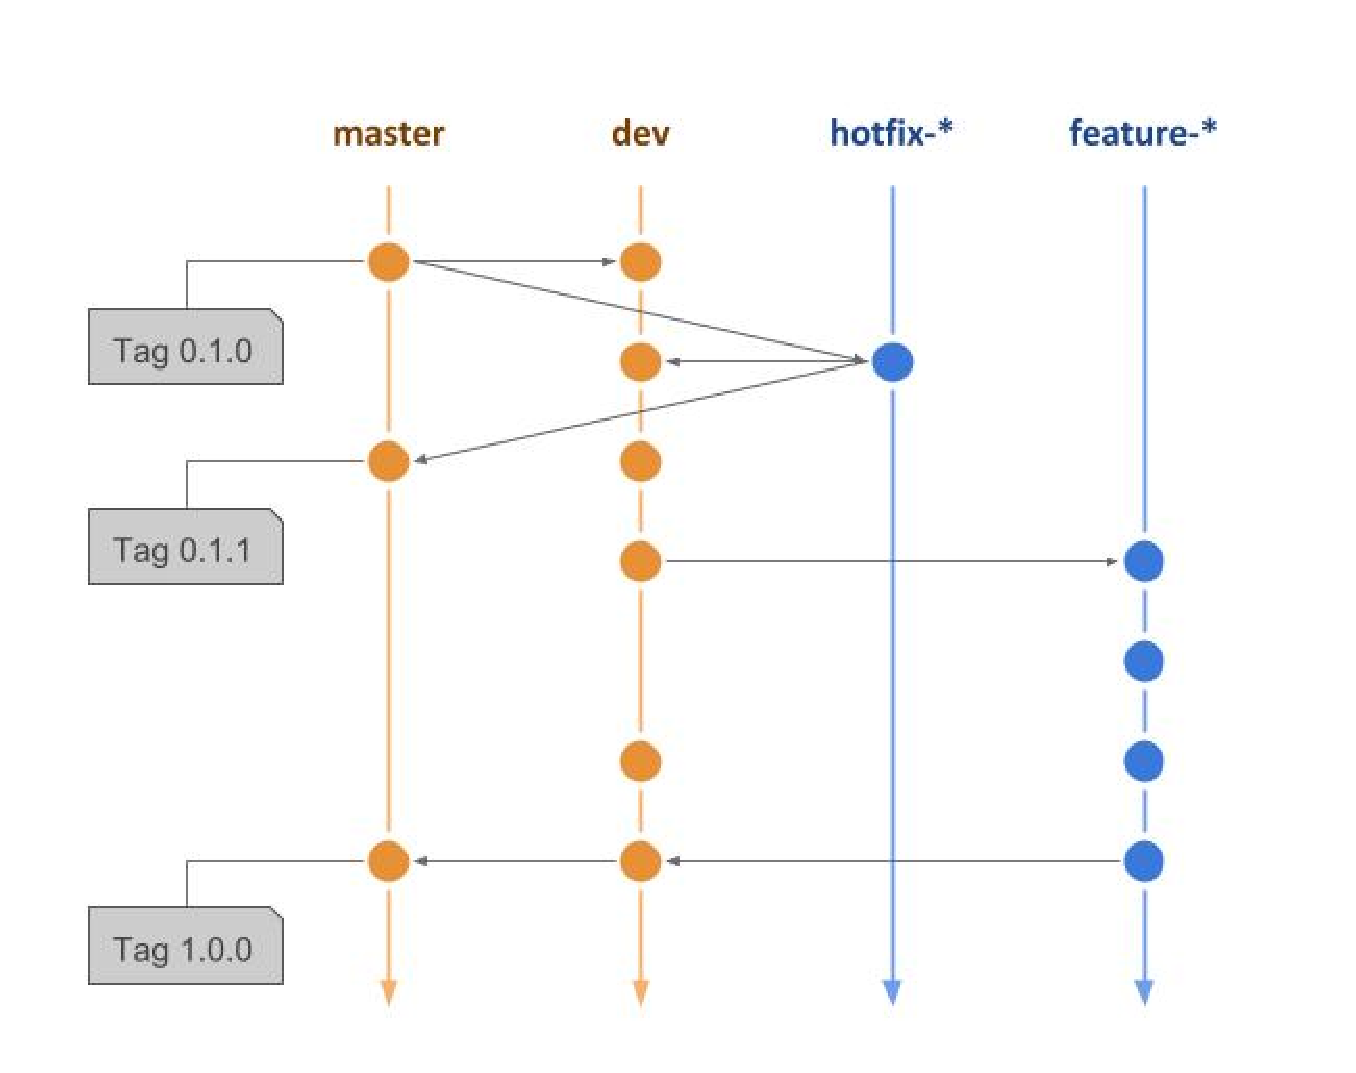
\includegraphics[width=0.8\textwidth]{figuras/controle_versao}
  \caption{Controle de versão do Cupper}
  \label{fig:ctrl_versao}
\end{figure}

Neste modelo, as principais \textit{branchs} tem o tempo de vida infinito, ou seja,
em nenhum momento são removidas do repositório remoto. São elas:

\begin{itemize}
  \item \textit{master}: reflete o estado de \lq\lq pronto para produção\rq\rq,
    ou seja, estabelece uma versão estável do sistema. Todo
    o trabalho realizado, em algum ponto do desenvolvimento
    deve ser integrado a esta \textit{branch};
  \item \textit{dev}: onde ocorre a integração de todos os componentes,
    funcionalidades e correções. Contém todos os itens mais
    recentes desenvolvidos e é considerado a versão instável
    do sistema, ou seja, pode conter comportamentos indesejados
    e \textit{bugs} desconhecidos.
\end{itemize}

Há também as \textit{branches} de suporte que tem o tempo de vida curto, ou seja,
assim que concluídas, devem ser removidas do repositório remoto. São
elas:

\begin{itemize}
  \item \textit{feature}: deve ser ramificada da \textit{branch dev} e
    integrada a \textit{branch dev} quando finalizada. Contém todos os
    novos itens desenvolvidos para a nova funcionalidade;
  \item \textit{hotfix}: deve ser ramificada da \textit{branch master} e
    integrada a \textit{branch dev} e \textit{master} quando finalizada. São
    as correções que são realizadas na versão estável do sistema, e geralmente
    são pontos críticos que devem ser corrigidos imediatamente. Quando finalizadas
    deve-se criar uma \textit{tag} da versão estável do sistema;
\end{itemize}

\section{Coleta e Análise de Resultados}

Nesta seção será apresentado o método de coleta e análise dos resultados deste
trabalho para validação da proposta. Como disposto nos objetivos (\ref{sec:obj}),
o resultado da execução do Cupper é um \textit{script} em formato de receita Chef.
Tal receita poderá ser utilizada pelo Chef para replicar o ambiente. Sendo assim
O foco da coleta e análise de dados está na capacidade de replicar um ambiente
utilizando o Cupper e Chef de maneira automatizada.

Divide-se a coleta e análise de dados em quatro etapas:

\textbf{Etapa 1}: Nesta etapa será coletado os dados sobre quais informações o Cupper consegue
extrair e quais são as replicações. A coleta será feita por um \textit{checklist} que contenha
todos os itens propóstos para implementação da ferramenta. O \textit{checklist} será
utilizado para delimitar os dados base que serão coletados do ambiente para
a validação. Também é um informativo sobre até qual ponto o projeto conseguiu
alcançar.

\textbf{Etapa 2}: Nesta etapa será construído um ambiente que seja possível extraír as configurações
sem a utilização do Cupper. Essas informações estarão alinhadas ao \textit{cehcklist} da etapa
anterior e serão a base para o comparativo com o ambiente replicado.

\textbf{Etapa 3}: Nesta etapa a ferramenta Cupper irá ser executada no ambiente construído na etapa
anterior. As receitas geradas serão usadas pelo Chef em um ambiente limpo que contenha
apenas as configurações mínimas para o seu funcionamento, ou seja, um sistema
operacional (Debian ou Arch), acesso por interface de rede e o Chef (a seção
~\ref{sec:chef} define o ambiente mínimo para o funcionamento do Chef).

\textbf{Etapa 4}: Nesta etapa é feito a extração sem utilização do Cupper, assim como foi realizado
na etapa 2, no ambiente replicado. Então será feito uma comparação das configurações
dos dois ambientes.

A conclusão dos dados coletado e analizados será realizado pela porcentagem de
item correspondendes dos ambientes como demonstrado na tabela \ref{tab:ex_result}.

\begin{table}[H]
  \centering
  \setlength\extrarowheight{5pt}
  \begin{tabular}{|c|c|c|c|}
    \hline
    \rowcolor[HTML]{EFEFEF} 
  \textbf{Camada}                      & \textbf{\begin{tabular}[c]{@{}c@{}}Ambiente\\ (Extração Manual)\end{tabular}} & \textbf{\begin{tabular}[c]{@{}c@{}}Ambiente Replicado\\ (Extração Manual)\end{tabular}} & \multicolumn{1}{l|}{\cellcolor[HTML]{EFEFEF}\textbf{Replicado}} \\ \hline
                                         & Pacote Nginx Instalado                                                        & Pacote Nginx Instalado                                                                  & X                                                               \\ \cline{2-4} 
                                         & Configuração Nginx Aplicada                                                   & Configuração Nginx Aplicada                                                             & X                                                               \\ \cline{2-4} 
    \multirow{-3}{*}{Aplicação} & Pacote PostgreSQL Instalado                                                   & Pacote PostgreSQL Instalado                                                             & X                                                               \\ \hline
    Serviço                     & Serviço Nginx Executando                                                      & Serviço Nginx Não Executando                                                            &                                                                 \\ \hline
    \multicolumn{3}{|c|}{Porcentagem Replicada}                                                                                                                                                                    & 75\%                                                            \\ \hline
  \end{tabular}
  \caption{Exemplo de tabela de comparação dos resultados.}
  \label{tab:ex_result}
\end{table}

A extração manual será feita com a utilização de \textit{scripts bash}. O motivo da utilização desse
método é a necessidade de obter os dados de forma imparcial, ou seja, as informações extraídas
para a comparação não podem ser realizadas pelo Cupper ou Ohai, visto que estes são parte
do processo de extração e configuração do ambiente replicado e não podem ser utilizados para
validar a si mesmo.


